
\chapter*{Függelék}
\section*{Párhuzamos iperf mérés kódja}
\lstinputlisting{example.py}

\section*{AS gráf}
A gráf csomópontjai az internetet alkotó autonóm rendszerek (AS), a köztük lévő irányított élek a TMIT gépei felé vezető útvonalak, amelyek vastagsága azt mutatja hány különböző ip cím pár lett regisztrálva mint átlépő pont a két AS között.

\bigskip
\bigskip


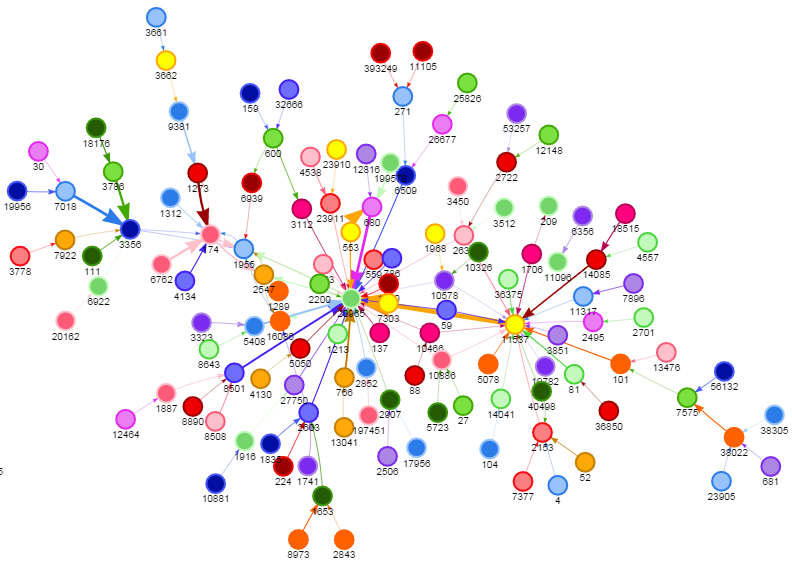
\includegraphics[width=1\textwidth,keepaspectratio]{figures/as-graph.png}